%\section{Aerial Computing: Dream of an intelligent sky}

\section{Introduction}

Unmanned aerial vehicles (a.k.a drones) are becoming an important part of our technological society. With myriad use cases, such as in sports photography~\cite{drone-sports1}, surveillance~\cite{drone-surveillance}, disaster management, search and rescue~\cite{disaster-drone,nepal-earthquake-drone}, transportation and package delivery~\cite{Amazondel:online,CSD-Amazon-Drone-patents,drone-package-delivery-google}, and more, these unmanned aerial vehicles are on the cusp of demonstrating their full potential. 

Hence, drones are rapidly increasing in number. Between 2015, when the U.S. Federal Aviation Administration (FAA) first required every owner to register their drone, and 2017, the number of drones has grown by over 200\%. At the time of writing, the FAA indicates that there are over 900,000 drones registered with the FAA drone registry database (\Fig{fig:faa-registrations}). By 2021, the FAA expects this number will exceed 4 million units~\cite{faa-2021}. Such an upward trend can be explained by the new opportunities that unmanned aerial vehicles are enabling.

% For example, by replacing the traditional forms of data collection from farming to project management on the construction site, drones have been reported to increase the time saving by 5-20X and hence reducing the costs up to 5X~\cite{dronedeploy:online}.

\begin{figure}[t!]
  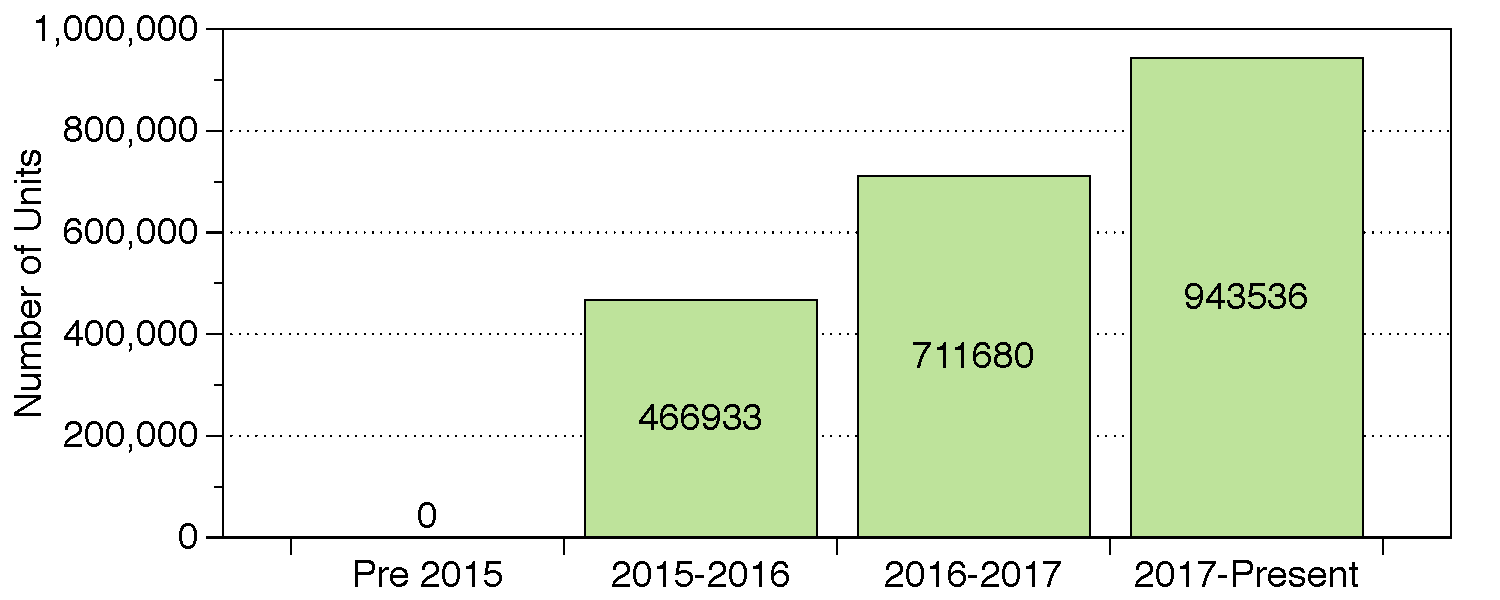
\includegraphics[trim=0 0 0 -10, clip, width=1.0\columnwidth]{figs/faa}
  \caption{Rapidly growing interest in UAVs. Data mined from FAA vehicle registration. The number of FAA registrations increased by 2X over the past two years, and it is rapidly growing. The FAA projects that by 2021 the number will exceed 4M units~\cite{FAA:online}.}
  \label{fig:faa-registrations}
\end{figure}


%\red{What are the big technical problems with drones} \lipsum[1]

The growth and significance of this emerging domain of autonomous agents call for architects attention. Challenges such as low endurance (how long the drone can last in the air) and small battery capacities for drones demand hardware and system architects' attention. The limited on-board energy budget manifests itself in the limited endurance and range of drones. This can be seen in various off-the-shelf commercial drones where endurance is typically less than 20 minutes, and flight range is about 15 miles~\cite{CSD-Amazon-Drone-patents}. To practically deploy drones, both their endurance and range must be improved. 

%\red{What should architects do here to help with the technical problems and what do they typically require here} \lipsum[1]

In this paper, we investigate and show the role of computing given the endurance and range challenges. For example, we show how a powerful compute subsystem can be deployed to mitigate the problem of limited endurance. The drone's compute subsystem dictates how fast a drone can maneuver, fly, and efficiently finish its mission. Hence, a computing subsystem that takes a long time to do path planning while the drone is hovering in the air, results in the inefficient consumption of energy. Furthermore, a more powerful compute subsystem can lead to more intelligent decision making (e.g., shorter paths to take). It is important to note that enabling intelligence on drones is challenging because of the computational power, size, weight, and cooling limitations.

%\red{Explain HILS and MAVBench goals} \lipsum[1]

To enable research and investigation, the foremost challenge to address is the lack of systematic benchmarks and infrastructure for research. To address this shortcoming, we introduce MAVBench, the first of its kind, a platform for the holistic evaluation of aerial agents, involving a closed-loop simulation framework and a benchmark suite. MAVBench facilitates the integrated study of performance and energy efficiency of not only the compute subsystem in isolation but also the compute subsystem's dynamic and runtime interactions with the simulated micro-aerial vehicle (MAV) as a whole.

%\red{Deep dive into the simulator -- one para} \lipsum[1]

The goals of MAVBench, which builds on top of AirSim~\cite{Airsim_paper}, are to faithfully capture all the interactions a real MAV encounters in the field and to ensure reproducible runs across experiments, starting from the software layers down to the hardware layers. Our simulation setup uses a hardware-in-the-loop configuration that can enable hardware and software architects to perform co-design studies to optimize system performance by considering the entire vertical application stack running on top of it, which includes the Robotics Operating System (ROS) and complete applications. It reports a variety of quality-of-flight (QoF) metrics, such as the performance, power consumption, and trajectory statistics of the drone.

%\red{Explain what MAVBench contains and why it is useful} \lipsum[1]
MAVBench provides an application suite covering a variety of popular applications of micro aerial vehicles. We constructed five distinct and widely used applications: \bench{Scanning}, \bench{Package Delivery}, \bench{Aerial Photography}, \bench{3D Mapping} and \bench{Search and Rescue.} MAVBench applications are whole, comprised of holistic end-to-end application dataflows found in a typical real world drone application. These applications' dataflows are comprised of several state-of-the-art computational kernels, such as object detection~\cite{yolo16,hog}, occupancy map generation~\cite{octomap}, motion planning~\cite{ompl}, localization~\cite{orbslam2,vins-mono}, which we integrated together to create complete applications. MAVBench has the ability to ``plug and play'' different computational kernels to study trade-offs for the same task.

%\red{What are some of the research observations we make} \lipsum[1]

MAVBench enables us to investigate, understand and quantify the power and performance demands of typical MAV applications from the underlying compute subsystem. More specifically, it allows us to answer a very fundamental question: \emph{what is the role of computing in autonomous MAVs?} 

We quantitatively demonstrate via simulations and measurements that compute has a significant impact on how efficiently the drone uses its energy while flying, affecting mission times and overall energy consumption. An off-the-shelf MAV, such as the DJI~Matrice~\cite{dji-matrice} or \solo~\cite{solo3DR}, consumes between 300~W to 400~W for its rotors, as much power as a typical data center server, with an average endurance that is typically less than 20 minutes. Compute on average consumes less than 5\% of that total system power.  A state-of-the-art compute platform like the Nvidia TX2 consumes about 10~W on average. However, the compute performed onboard by the TX2 can affect flight mission time by as much as 2X. We conduct frequency and core scaling experiments on the TX2 to demonstrate how the \emph{compute performance affects the drone's velocity, which in turns impacts its mission time, and consequentially the drone's total system energy consumption.}

Taking advantage of our platform, we provide three case studies targeting performance, energy and reliability. The performance case study examines a sensor-cloud architecture for drones where the computation is distributed across the edge and the cloud. Such an architecture shows a reduction in the drone's overall mission time by as much as 50\% when the cloud support is enabled. The energy case study, targets Octomap~\cite{octomap}, a computationally intensive kernel that is at the heart of some of the MAVBench applications and demonstrates how approximations in its internal representation, and thus compute, can enable safe flight while improving overall energy consumption. Last by not least, our reliability case study investigates the impact of sensor noise on the performance of one of our applications, namely package delivery, showing a performance degradation of up to 90\% while in presence of high depth image noise. All three case studies demonstrate the potential ways in which MAVBench can be used for architecture and systems research. In general, the platform allows a variety of hardware and software (co-)design studies.

%OctoMap generates a volumetric 3D model of its environment that the collision avoidance and motion planning task use to ensure a safe flight. By dynamically adjusting OctoMap's ``resolution'' (i.e., perception) of the environment, we can control the amount of computing performed for a trade off in accuracy. Expediting OctoMap processing leads to faster real-time decision making and max safe velocity. This allows the drone to fly faster and complete its mission with more energy remaining in its battery. 

In summary, we make the following contributions:

\begin{itemize}
    \item We present a closed-loop simulation framework that enables hardware and software architects to perform performance and power optimization studies that are relevant to computer system design and architecture.
    \item We introduce an end-to-end benchmark suite, comprised of several workloads and their corresponding state-of-the-art kernels. These workloads represent popular real-world use cases of MAVs.
    \item We uncover the role of computing and its relationship with flight time and endurance for unmanned MAVs.
    \item We present case studies to concretely explore and emphasize compute's impact on performance, energy and reliability of MAV systems.

\end{itemize}


\begin{comment}


Furthermore, on the road to intersect with the proliferation of drones is the interest in making these aerial systems fully autonomous~\cite{gopalakrishnan2016countermeasures}. There is growing interest in equipping drones with more intelligence using recent advancements in AI and machine learning. One of the primary motivations for adding these capabilities is to eliminate the human in the loop. Human operators are an unreliable source of operation. Over 85\% of general aviation crashes are caused by pilot error~\cite{li2001factors,shkrum1996fatal}.


This paper is an attempt to present an architectural overview of aerial agents, and further provide tools to study them, namely, a simulation platform and a benchmark. In addition, we conduct various case-studies using aforementioned tools, and show invaluable conclusions such tools enable. More concretely, our contributions are three fold:
	  \begin{itemize} 
       \item A closed-loops end-to-end simulation environment as a necessity to probe into the extra-system (system/environment) and intra-system interactions. Case studies are further presented to show how ignoring such interactions can be detrimental to design and development of aerial systems and hence platforms without such probing capabilities should be abandoned (section 3). 
      \item Mav-bench: A new and diverse benchmark suit targeting aerial computing enabling architects for characterization/design and development of aerial agents (section 4 and 5).
	\item  unraveling the non-traditional compute/energy relationship existing for such systems. Concrete ways in which compute can affect the overall systems energy and in-turn agents mission success is studied and presented (section 6)
      \end{itemize}
   
\end{comment}

The rest of the paper is organized as follows. 
%\Sec{sec:background} gives background on UAVs and MAVs that is relevant to this paper. 
~\Sec{sec:background} provides basic background about Micro Aerial vehicles, the reasons for their prominence amongst UAVs, and the challenges system designers face.  \Sec{sec:simulation} describes the MAVBench closed-loop simulation platform. \Sec{sec:mavbench} introduces the MAVBench benchmark suite and describes the computational kernels and full-system stack it implements. \Sec{sec:char} uses MAVBench to uncover an interesting relationship between compute and the MAV's total system energy consumption. \Sec{sec:case-study} presents three case studies further examining the impact of compute stack on performance, energy and reliability of MAV systems. \Sec{sec:related} discusses related work, and \Sec{sec:conclusion} summarizes and concludes the paper.
       